\documentclass[aspectratio=169,t,11pt,table]{beamer}
\usepackage{../../slides}
\usepackage{../../math}
\usepackage{../../uark_colors}
\definecolor{accent}{HTML}{9D2235}
\definecolor{accent2}{HTML}{2B5269}

\title{Topic 3: Simple Linear Regression}
\subtitle{\it  ECON 4753 — University of Arkansas}
\date{Fall 2024}
\author{Prof. Kyle Butts}

\begin{document}

% ------------------------------------------------------------------------------
\begin{frame}[noframenumbering,plain]
\maketitle

% \bottomleft{\footnotesize $^*$A bit of extra info here. Add an asterich to title or author}
\end{frame}
% ------------------------------------------------------------------------------

\section{Bivariate Regression}

\begin{frame}{Covariance and Correlation}
  Recall the ways we discussed relationships between two random variables $X$ and $Y$:

  \bigskip
  Covariance, $\sigma_{XY}$ (sample analogue: $s_{XY}$)
        
  \begin{itemize}
    \item Direction matters, but magnitude is hard to interpret
  \end{itemize}
        
  \bigskip
  Correlation, $\rho_{XY}$ (sample analogue: $r_{XY}$)
  
  \begin{itemize}
    \item Direction and magnitude matter
    
    \item Correlation is always value between $[-1, 1]$
  \end{itemize}
\end{frame}

\begin{frame}{Covariance and Correlation}
  The \alert{correlation} is calculated as
  \begin{equation}\label{eq:correlation}
    r = \frac{Cov(X, Y)}{\sqrt{Var(X)} \cdot \sqrt{Var(Y)}}
  \end{equation}

  \begin{itemize}
    \item Correlation is a function of covariance, just normalizes the magnitudes so we can interpret.
  \end{itemize}
\end{frame}

\begin{frame}{Practice question}
  Suppose you calculate the sample covariance, $s_{XY} = 1.2$, and the sample standard deviations $s_X = 2$ and $s_Y = 2.5$. What is the sample correlation, $r_{XY}$?

  \begin{itemize}
    \item $0.0576$
    \item $0.24$
    \item $0.048$
    \item $4.17$
  \end{itemize}
\end{frame}


\begin{frame}{Relationship between X and Y}
  Consider this plot of NYC Math and Reading SAT Scores\only<2>{. The easiest way to summarize the relationship between $X$ and $Y$ is using a \alert{regression line}, aka the ``line of best fit''.}
  
  \medskip
  \begin{center}
    \only<1>{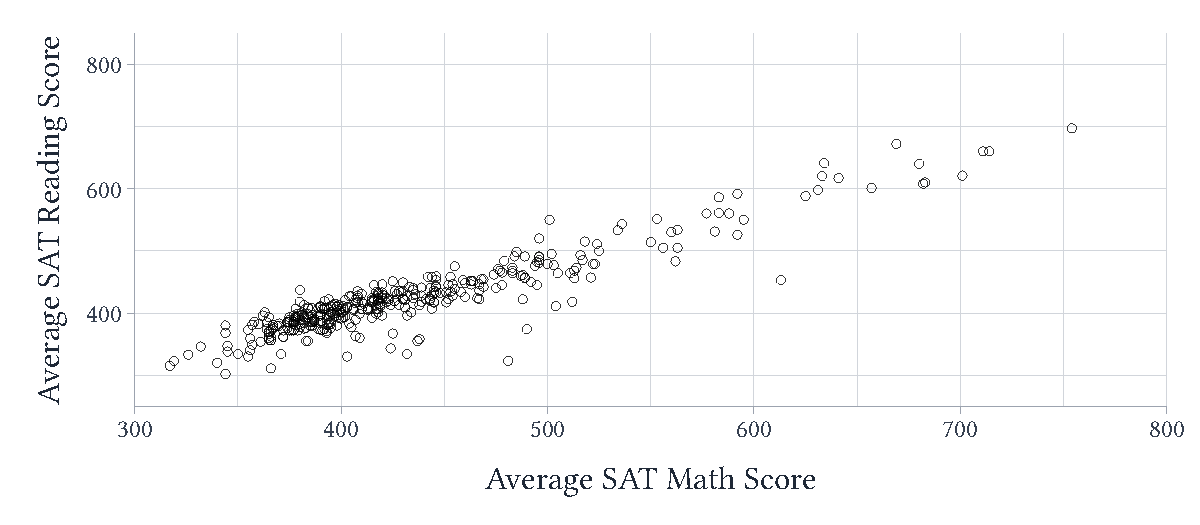
\includegraphics[width = 0.8\textwidth]{figures/nyc_sat_raw_data.pdf}}
    \only<2>{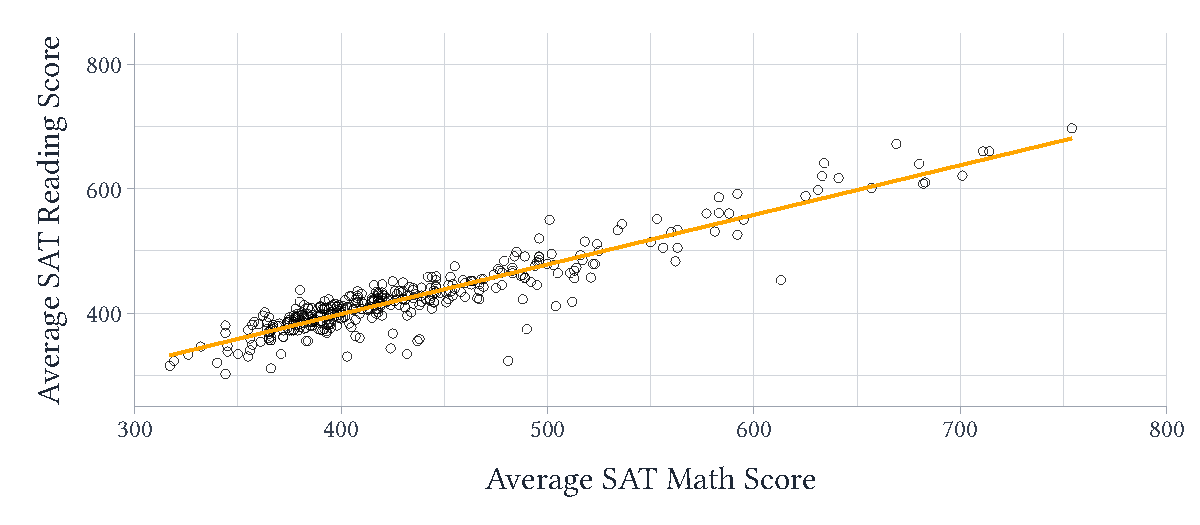
\includegraphics[width = 0.8\textwidth]{figures/nyc_sat_reg_line_of_best_fit.pdf}}
  \end{center}
\end{frame}

\begin{frame}{Regression line}
  We can write this linear model as 
  $$
    y = f(X) + \varepsilon = \beta_0 + \beta_1 * X + \varepsilon
  $$
  
  \bigskip
  The model says $y$ is a linear function of $X$. $\beta_0$ is the `intercept' and $\beta_1$ is the `slope' of the line. 
  
  \pause
  \bigskip
  We use the following terminology:
  \begin{itemize}
    \item $y$ is called `the dependent variable', `the response variable', or `the predicted variable' 
    
    \item $X$ is called `the independent variable', `the explanatory variable', `the control variable', or `the predictor variable'
  \end{itemize}
\end{frame}

\begin{frame}{Motivation for regression line}
  \vspace*{-2\bigskipamount}
  $$
    y = \beta_0 + \beta_1 * X + \varepsilon
  $$

  There are a few advantages to using a line:
  \begin{enumerate}
    \item Often time does a good job at prediction (like in our NYC example)
    \item Easy to interpret 
    \item A simple model faces less risk of overfitting the data.
  \end{enumerate}

  \bigskip
  The cost is that the model might be \emph{too simplistic} and fail to caputure many non-linear relationships between $X$ and $y$. It might yield poor predictions.
\end{frame}

\begin{frame}{Regression Line Example}
  In the previous example, the regression `line of best fit' (we will talk about how to find this line later) is given by 
  $$
    \widehat{\text{Average SAT Reading}} = 78.87 + 0.7983 * \text{Average SAT Math}
  $$
  
  The $\widehat{\quad}$ symbol means that we are \emph{predicting} average SAT reading score with our model
\end{frame}


\begin{frame}{Regression Line Example}{Predictions}
  If a school has an average SAT math score of 600, we would predict their SAT reading score would be 
  $$
    \widehat{\text{Average SAT Reading}} = 78.87 + 0.7983 * 600 = 557.85
  $$

  \pause 
  That is, our linear model would predict an average SAT reading score of 558.
\end{frame}

\begin{frame}{Slope of Line}
  How does $y$ change with $X$? Take $X$ and $X + 1$, we have the following predicted values:
  $$
    \hat{y} = \beta_0 + \beta_1 X \quad\text{ and }\quad 
    \hat{y}_{\text{new}} = \beta_0 + \beta_1 (X + 1)
  $$

  \bigskip
  So $y$ changes by 
  \begin{align*}
    \Delta y &= \left[ \beta_0 + \beta_1 (X + 1) \right] - \left[ \beta_0 + \beta_1 X \right] \\
    &= \beta_1 X + \beta_1 - \beta_1 X \\ 
    &= \beta_1
  \end{align*}

  \bigskip
  $\implies$ marginal effect of $X$ on $y$ is constant and equal to $\beta_1$
\end{frame}

\begin{frame}{Slope of Line}{Example of Constant Marginal Effects}
  \vspace*{-2\bigskipamount}
  $$
    \text{Wage} = \beta_0 + \beta_1 \text{ Education} + \varepsilon
  $$

  Implies that each year of education leads to the same change in wages
  \begin{itemize}
    \item Do you think that is reasonable?
    
    \pause
    \item Might there be a jump at high-school degree (``signaling'')?
    
    \item Returns to schooling might get smaller as we get more educated?
  \end{itemize}
\end{frame}



\begin{frame}{Prediction Error}
  Given our line, we will want to be able to evaluate how good our model does at predicting observations $y$

  \bigskip
  Define the \alert{prediction error} as 
  $$
    \hat{\varepsilon} = \underbrace{y}_{\text{true value}} - \underbrace{\hat{y}}_{\text{predicted value}} 
  $$

\end{frame}

\begin{frame}{Prediction Error}
  In the case of a linear prediction model
  $$
    \hat{\varepsilon} = \underbrace{y}_{\text{true value}} - \underbrace{\hat{y}}_{\text{predicted value}} = y - b_0 - b_1 X,
  $$
  where $b_0$ and $b_1$ are any numbers (for now).

  \bigskip
  Large $\hat{\varepsilon}$ mean you did a poor job of predicting that observation. That could be because
  \begin{enumerate}
    \item The linear model is bad at predicting $y$
    \item Or, the true noise $\varepsilon$ is making $y$ far away from the systematic component $f(X)$.
  \end{enumerate}
\end{frame}


\begin{frame}{Mean-square Error}
  Just like in Topic 2, we can form the mean-square prediction error of our linear model (in our training sample):
  $$
    \text{MSE} = \frac{1}{n} \sum_{i=1}^n (y_i - b_0 - b_1 X_i)^2
  $$

  \bigskip
  A line does a good job at predicting if MSE is (relatively) small. 

  \pause
  \bigskip
  What if we select a line based on making mean-squared prediction error as small as possible?
\end{frame}

\imageframe{figures/nyc_sat_ex_mspe_1.pdf}
\imageframe{figures/nyc_sat_ex_mspe_2.pdf}
\imageframe{figures/nyc_sat_ex_mspe_3.pdf}
\imageframe{figures/nyc_sat_ex_mspe_ols.pdf}

\begin{frame}{``Least Squares'' Regression}
  This is the basis for the \alert{ordinary least squares} regression estimator:

  $$
    \min_{\hat{\beta}_0, \hat{\beta}_1} \frac{1}{n} \sum_{i=1}^n (y_i - \hat{\beta}_0 - \hat{\beta}_1 X_i)^2
  $$

  \pause
  \bigskip
  $\hat{\beta}_0$, $\hat{\beta}_1$ are the values of the intercept and slope that minimize prediction error
  \begin{itemize}
    \item Do you see where the term ``least squares'' comes from?
  \end{itemize}
\end{frame}

\begin{frame}{Deriving Least Squares Formula}
  To minimize the function, we will take derivatives with respect to $\hat{\beta_0}$ and $\hat{\beta_1}$ and set equal to zero. First, $\hat{\beta_0}$:
  \begin{align*}
    \frac{\partial}{\partial \hat{\beta_0}} \sum_{i=1}^n (y_i - \hat{\beta_0} - \hat{\beta_1} X_i)^2 &= 0 \\
    \pause
    \implies \sum_{i=1}^n 2 (y_i - \hat{\beta_0} - \hat{\beta_1} X_i) &= 0 \\
    \implies \sum_{i=1}^n \hat{\varepsilon}_i &= 0
  \end{align*}
\end{frame}

\begin{frame}{Deriving Least Squares Formula}
  Continuing our first-order conditions for $\hat{\beta}_0$: $0 = \sum_{i=1}^n 2 (y_i - \hat{\beta_0} - \hat{\beta_1} X_i)$
  \begin{align*}
    0 &= \sum_{i=1}^n 2 (y_i - \hat{\beta_0} - \hat{\beta_1} X_i) \\
    \implies 0 &= \left(\sum_{i=1}^n y_i \right) - n \hat{\beta_0} - \left( \sum_{i=1}^n \hat{\beta_1} X_i \right) \\ 
    \pause
    \implies n \hat{\beta_0} &= \left(\sum_{i=1}^n y_i \right) - \left( \sum_{i=1}^n \hat{\beta_1} X_i \right) \\ 
    \pause
    \implies \hat{\beta_0} &= \frac{1}{n} \left(\sum_{i=1}^n y_i \right) - \hat{\beta_1} \frac{1}{n} \left( \sum_{i=1}^n X_i \right) \\ 
  \end{align*}
\end{frame}

\begin{frame}{Deriving Least Squares Formula}
  All our work lead to
  \begin{align*}
    \hat{\beta_0} = \frac{1}{n} \left(\sum_{i=1}^n y_i \right) - \hat{\beta_1} \frac{1}{n} \left( \sum_{i=1}^n X_i \right) 
  \end{align*}  

  \bigskip 
  This we can write as our first least-squares formula
  $$\hat{\beta_0} = \bar{y} - \hat{\beta_1} \bar{X}$$
\end{frame}


\begin{frame}{Deriving Least Squares Formula}
  To minimize the function, we will take derivatives with respect to $\hat{\beta_0}$ and $\hat{\beta_1}$ and set equal to zero. Second, $\hat{\beta_1}$:
  \begin{align*}
    \frac{\partial}{\partial \hat{\beta_1}} \sum_{i=1}^n (y_i - \hat{\beta_0} - \hat{\beta_1} X_i)^2 &= 0 \\
    \pause
    \implies \sum_{i=1}^n 2 X_i (y_i - \hat{\beta_0} - \hat{\beta_1} X_i) &= 0 \\
    \pause
    \implies \sum_{i=1}^n X_i \hat{\varepsilon}_i &= 0
  \end{align*}
\end{frame}

\begin{frame}{Deriving Least Squares Formula}
  Taking $\hat{\beta_0} = \bar{y} - \hat{\beta_1} \bar{X}$ and plugging into our first order condition for $\hat{\beta}_1$:
  \begin{align*}
    0 &= \sum_{i=1}^n X_i (y_i - \hat{\beta_0} - \hat{\beta_1} X_i) \\
    \implies 0 &= \sum_{i=1}^n X_i (y_i - \bar{y} + \hat{\beta_1} \bar{X} - \hat{\beta_1} X_i) \\
    \pause
    \implies 0 &= \sum_{i=1}^n X_i \left( \left( y_i - \bar{y} \right) + \hat{\beta_1} \left( \bar{X} - X_i \right) \right) \\
    \implies 0 &= \sum_{i=1}^n X_i \left( y_i - \bar{y} \right) - \hat{\beta_1} \sum_{i=1}^n X_i \left( X_i - \bar{X} \right) \\
  \end{align*}
\end{frame}

\begin{frame}{Deriving Least Squares Formula}
  \begin{align*}
    0 &= \sum_{i=1}^n X_i \left( y_i - \bar{y} \right) - \hat{\beta_1} \sum_{i=1}^n X_i \left( X_i - \bar{X} \right) \\
    \smallskip
    \implies \hat{\beta}_1 &= \frac{\sum_{i=1}^n X_i \left( y_i - \bar{y} \right)}{\sum_{i=1}^n X_i \left( X_i - \bar{X} \right)}
  \end{align*}

  With a bit of algebra, you can find:
  \begin{align*}
    \hat{\beta}_1 = \frac{\frac{1}{n} \sum_{i=1}^n \left( X_i - \bar{X} \right) \left( y_i - \bar{y} \right)}{\frac{1}{n} \sum_{i=1}^n \left( X_i - \bar{X} \right)^2} = \frac{\cov(X, y)}{\var(X)}
  \end{align*} 
\end{frame}

\begin{frame}{Least Squares Formula}
  With that, we have a formula for OLS coefficients:
  $$
    \hat{\beta}_1 = \frac{\cov(X, y)}{\var(X)} \quad\text{ and }\quad \hat{\beta}_0 = \bar{y} - \hat{\beta_1} \bar{X}
  $$

  \pause
  \bigskip
  Note that the slope $\hat{\beta}_1$ describes how $y$ changes with $X$
  \begin{itemize}
    \item That is what the covariance tells us!
  \end{itemize}
\end{frame}

\begin{frame}{Least Squares example}
  \vspace*{-\bigskipamount}
  $$
    \hat{\beta}_1 = \frac{\cov(X, y)}{\var(X)} \quad\text{ and }\quad \hat{\beta}_0 = \bar{y} - \hat{\beta_1} \bar{X}
  $$

  In our NYC example, calculate the regression coefficients of $y = $ Average SAT Reading Score and $X = $ Average SAT Math Score by hand. Here are the following statistics:
  
  
  $\cov{X, y} = 4132.97$

  $\var{X} = 5177.14$

  $\bar{X} = 432.94$

  $\bar{y} = 424.50$


  \pause
  % TODO: Answer
\end{frame}

\begin{frame}{Interpreting a Regression}

  $$
  y = \beta_0 + \beta_1 X
  $$

  \begin{itemize}
    \item $\beta_0$ is the value of $y$ whenever $X = 0$.
    
    \item $\beta_1$ is the amount $y$ changes when $X$ increases by one.
  \end{itemize}
\end{frame}

\begin{frame}{Interpreting a Regression}
  Consider this hypothetical regression:
  $$
    \hat{\text{Wins}}_i = 20.783 + 0.00913 * \text{ 3-point shots}
  $$
  
  \bigskip
  Our intercept, 20.783, is the predicted number of wings for an NBA team that shoots no 3-point shots
  
  \pause
  \bigskip
  Our slope, 0.00913, is the number of additional wins predicted for every 1 shot increase in the number of per-game 3-point shots
\end{frame}

\begin{frame}{Interpreting a Regression}
  Say we calculate the following regression line from hours studied and final exam grades:
  $$
    \widehat{\text{Final Exam}} = 38 + 5.7 * \text{Hours of Studying}
  $$

  Interpret the two regression coefficients
  \pause

  \begin{itemize}
    \item 38 is the predicted score with no studying.
    \pause
    \item Each hour of studying increases the predicted final exam score by 5.7 points.
  \end{itemize}
\end{frame}

\begin{frame}{Practice Question}
  Given that same regression line, $\widehat{\text{Final Exam}} = 38 + 5.7 * \text{Hours of Studying}$, what is the predicted final exam score if you study 8 hours?

  \pause 
  $38 + 5.7 * 8 = 83.6$
\end{frame}

\begin{frame}{Practice Question}
  A convenience store calculates a least squares line that describes how price (in dollars) of juuls affects the quantity sold; 
  $$
    \widehat{\text{Juuls sold}} = 117 - 12.4 * \text{price}
  $$ 

  If price \emph{decreases} by 1 dollar, what happens to number of juuls sold?

  \pause
  Quantity decreases by 12.4 units
\end{frame}



\begin{frame}{Algebraic properties of OLS}
  There are three properties of OLS we will cover. The first two are our first-order conditions
  \begin{enumerate}
    \item $\sum_{i=1}^n \hat{\varepsilon}_i = 0$
    \begin{itemize}
      \item The residuals sum to $0$
    \end{itemize}

    \pause
    \medskip
    \item $\sum_{i=1}^n X_i \hat{\varepsilon}_i = 0$
    \begin{itemize}
      \item The residual is uncorrelated with the $X$ variable
    \end{itemize}
    
    \pause
    \medskip
    \item $(\bar{X}, \bar{y})$ is on the regression line
  \end{enumerate}
\end{frame}

\begin{frame}{Algebraic properties of OLS}
  $(\bar{X}, \bar{y})$ is on the regression line comes from:
  \begin{align*}
    \bar{y} &= \frac{1}{n} \sum_{i=1}^n (\hat{\beta}_0 + \hat{\beta}_1 X_i + \hat{\varepsilon}_i) \\
    &= \hat{\beta}_0 + \hat{\beta}_1 \frac{1}{n} \sum_{i=1}^n X_i + \frac{1}{n} \sum_{i=1}^n \hat{\varepsilon}_i \\
    &= \hat{\beta}_0 + \hat{\beta}_1 \bar{X} + 0 \\
  \end{align*}
\end{frame}

\subsection{Prediction vs Causation}

\begin{frame}{Cautions about Correlation and Regression}
  Our regression line is fit by comparing individuals with larger and smaller $X$ values and seeing if units with larger $X$ have larger or smaller values of $y$. 

  \pause
  \bigskip
  Units with larger values of $X$ might have larger values of other variables and those other variables can affect $y$
  \begin{itemize}
    \item Which variable is driving the change in $y$? We do not know
  \end{itemize}

  Do not confuse \emph{prediction} with \emph{causation}!!! 
\end{frame}

\begin{frame}{Example of Prediction vs. Causation}
  Units with more years of schooling have higher wages
  \begin{itemize}
    \item Is this because of schooling?
    \item Or, is this because people with more schooling have higher intelligence? Differing home backgrounds? More responsible? 
  \end{itemize}

  \pause
  \bigskip\bigskip
  \begin{center}
    Correlation and regression are powerful tools for describing the relationship between two variables, but you must be careful! 
  \end{center}
\end{frame}

\begin{frame}{Correct regression interpretation}
  In general, you should use the following language:
  
  \begin{tcolorbox}[boxrule = 0pt, frame hidden, sharp corners, enhanced, borderline west = {4pt}{0pt}{green}, interior hidden]
    {\color{green}\Large $\checkmark$\ } Our regression model predicts that a one unit increase in $X$ is associated with a $\hat{\beta}_1$ units increase/decrease in $Y$
  \end{tcolorbox}

  \bigskip
  Do not say!!!!!! 
  \begin{tcolorbox}[boxrule = 0pt, frame hidden, sharp corners, enhanced, borderline west = {4pt}{0pt}{red}, interior hidden]
   {\color{red}\Large $\times$\ } Increase $X$ by one unit increases/decreases $Y$ by $\hat{\beta}_1$ units
  \end{tcolorbox}
\end{frame}

\begin{frame}{Learning about Causation}
  If you are interested in learning how to estimate \emph{causal effects}, you should take my Master's level class, ECON 5783 :-) 
\end{frame}


\section{Regression Inference}

\begin{frame}{Regression Inference}
  As we have seen, the regression coefficient $\hat{\beta}_1$ is often of interest
  \begin{itemize}
    \item Predicted change in $y$ when you increase $X$ by one unit
  \end{itemize}

  \pause
  \bigskip
  We want to be able to describe the uncertainty around this estimate. How does $\hat{\beta}_1$ change under repeated sampling?
  \begin{itemize}
    \item That is, what is the \emph{sampling distribution} of $\hat{\beta}_1$?
  \end{itemize}
\end{frame}

\imageframe{figures/ex_inference_orig_reg.pdf}
\imageframe{figures/ex_inference_extra_sample_1.pdf}
\imageframe{figures/ex_inference_extra_sample_2.pdf}
\imageframe{figures/ex_inference_extra_sample_5.pdf}
\imageframe{figures/ex_inference_extra_sample_100.pdf}

\begin{frame}{Regression Inference}
  For each sample of size $n$, the regression coefficient estimate $\hat{\beta}_1$ is different
  \begin{itemize}
    \item As $n$ gets large, the noise of the estimate should get smaller
  \end{itemize}
\end{frame}

\begin{frame}{Sample Distribution of Sample Mean}
  Recall that we have the sample distribution of the sample mean (provided $n$ is `big enough'):
  $$
    \bar{X}_n \sim \mathcal{N}(\mu, \frac{\sigma^2}{n})
  $$
  \begin{itemize}
    \item What is the equivalent for regression estimates?
  \end{itemize}
\end{frame}

\begin{frame}{Sample Distribution of Regression Coefficients}
  Say the true regression line is 
  $$
      y_i = \beta_{0,0} + X_i \beta_{1,0} + \varepsilon_i
  $$
  \begin{itemize}
    \item $\beta_{0,0}$ and $\beta_{1,0}$ denotes the true regression coefficient for the population
    
    \item $\varepsilon$ is the error term from the true regression line 
  \end{itemize}

  \pause
  \bigskip
  The sampling distribution of $\hat{\beta}_1$ (for $n$ `big enough') is:
  $$
    \hat{\beta}_1 \sim 
    \mathcal{N}\left( 
      \beta_{1, 0}, \frac{ \var{\varepsilon} / n }{\var{X}} 
    \right)
  $$
\end{frame}

\begin{frame}{Standard Error}
  $$
    \hat{\beta}_1 \sim 
    \mathcal{N}\left( 
      \beta_{1, 0}, \frac{ \var{\varepsilon} / n }{\var{X}} 
    \right)
  $$

  \bigskip
  With this, we can calculate the \alert{standard error}, i.e. the standard deviation of the sample distribution of $\hat{\beta}_1$:
  $$
    \text{SE}(\hat{\beta}_1) = \sqrt{ \frac{ \var{\hat{\varepsilon}} / n }{\var{X}} }
  $$
  \begin{itemize}
    \item We use the residual $\hat{\varepsilon}$ because we do not observe the true error term
  \end{itemize}
\end{frame}

\begin{frame}{Standard Error}
  $$
    \text{SE}(\hat{\beta}_1) = \sqrt{ \frac{ \var{\hat{\varepsilon}} / n }{\var{X}} }
  $$

  \begin{itemize}
    \item As our sample size gets larger, $n \to \infty$, we have the distribution converges to the true value (\emph{consistency})
  \end{itemize}
\end{frame}


\begin{frame}{Confidence intervals for $\hat{\beta}_1$}
  Since we have an approximately normally distributed random variable, we can form confidence intervals just like before:
  $$
    \left[
      \hat{\beta}_1 - 1.96 * \text{SE}(\hat{\beta}_1), 
      \hat{\beta}_1 + 1.96 * \text{SE}(\hat{\beta}_1)
    \right]
  $$

  \pause
  \bigskip
  The interpretation is as before: across repeated samples, 95\% of samples' confidence intervals will contain the true value $\beta_{1, 0}$.
\end{frame}

\begin{frame}{Confidence intervals for $\hat{\beta}_1$}

\end{frame}

% TODO: Regression in R and how to read the regression table
\begin{frame}{}

\end{frame}


\section{Goodness of Fit}

\begin{frame}{$R^2$}
  Next we define a measure to evaluate how well the regression line fits:
  $$
  \cranberry{R^2} = \frac{\sum_{i=1}^n (\hat{Y}_i - \bar{Y})^2}{\sum_{i=1}^n (Y_i - \bar{Y})^2}
  $$
\end{frame}

\begin{frame}{Intuition of $R^2$}
  Intuitively, $R^2$ measures the percent of variation in $Y$ explained by the model
  
  $$
    \cranberry{R^2} = \frac{
      \text{variation in } \hat{y} \text{ along the regression line as x varies}
    }{
      \text{total variation in observed values of y}
    }
  $$
\end{frame}

\imageframe{figures/r2_comparisons.pdf}


\begin{frame}{$r$ and $R^2$}
  Correlation, $r$, describes the strength of a straight-line relationship between two variables

  \bigskip
  $R^2$, is the fraction of the variation in the values of y that is explained by the least-squares regression of $y$ on $X$. In the case of a single-variable regression, we have 
  $$
    \cranberry{R^2} = r^2
  $$
\end{frame}

\begin{frame}{$r$ and $R^2$}
  Lets say we have $r = -0.7786$ and $\cranberry{R^2} = (-0.7786)^2 = 0.6062$ between exercise and weight loss. 
  
  \begin{itemize}
    \item $r = -0.7786$, there is a strong negative linear relationship between time exercised and amount of weight gained
    
    \item $\cranberry{R^2} = 0.6062$, about 61\% of the variation in weight losseis accounted for by the linear relationship between weight loss and exercise. This means about 39\% of the change in weight lossed is not explained by this relationship
  \end{itemize}
\end{frame}

\begin{frame}{$R^2$ Sidebar}
  A small $R^2$ does not mean the result is uninteresting. All it means is that the $x$ variable alone does not explain a large portion of the variation in $y$.
  
  \pause
  \bigskip  
  \textbf{Example:} You find a significant relationship between exercise and income, but it has a small $R^2$. 
  
  \medskip
  We know income is determined by a variety of variables -- parent's income, education, innate ability, experience, etc. 
  
  \begin{itemize}
    \item Your result isn't uninteresting; it just means there is a lot of variation in income \emph{not due} to exercise, which is exactly what we'd expect
  \end{itemize}
\end{frame}

\begin{frame}{$R^2$ Practice Question}
  Say a researcher calculated a correlation coefficient 0.503 between SAT scores and college freshman GPA. This implies an $R^2$ of 0.253. 
  
  \bigskip
  Practice interpreting what this $R^2$ mean? 
  \begin{itemize}
    \item Does this make sense? What other things could explain the variation in freshman year GPA?
  \end{itemize}
\end{frame}

\section{Influential Observations}

\begin{frame}{Influential Observations}
  Our regression line is sensitive to \alert{outliers}, either in the $X$ or $y$ dimension 
  \begin{itemize}
    \item We say an outlier is \alert{influential} if deleting it changes our regression line substantially
    
    \item The amount by which the line changes is called the \alert{leverage} an influential observation has
  \end{itemize}
\end{frame}

\imageframe{figures/nyc_sat_reg_line_of_best_fit.pdf}
\imageframe{figures/nyc_sat_outlier.pdf}

\begin{frame}{Outliers and large samples}
  % TODO
\end{frame}

\begin{frame}{Outliers}
  It is always good practice to \emph{plot} the raw data. In a world full of dirty data, you will be amazed at how quickly you can spot oddities in the data
  % TODO
\end{frame}


\section{\texorpdfstring{$\log$}{log} transformations}

% TODO








\end{document}
